\documentclass[12pt,a4paper]{article}

% Required Packages
\usepackage[utf8]{inputenc}
\usepackage[T1]{fontenc}
\usepackage{graphicx}
\usepackage{geometry}
\usepackage{hyperref}
\usepackage{titlesec}
\usepackage{booktabs}
\usepackage{caption}
\usepackage{subcaption}
\usepackage{float}
\usepackage{xcolor}
\usepackage{listings}
\usepackage{enumitem}
\usepackage{amsmath}
\usepackage{array}

% Layout Settings
\geometry{
    a4paper,
    total={170mm,257mm},
    left=25mm,
    top=25mm,
}

% Hyperlink Setup
\hypersetup{
    colorlinks=true,
    linkcolor=blue,
    filecolor=magenta,      
    urlcolor=cyan,
    pdftitle={GradeMinds AI: Agentic Learning Ecosystem},
}

% Section Formatting
\titleformat{\section}{\large\bfseries}{\thesection}{1em}{}
\titleformat{\subsection}{\normalsize\bfseries}{\thesubsection}{1em}{}

% --- Custom Title Page ---
\begin{document}

\begin{titlepage}
    \centering
    \vspace*{1cm}
    
    {\Huge \textbf{GradeMinds AI: An Agentic Learning Ecosystem}} \\[0.5cm]
    {\Large \textit{A Research-Driven Approach to Personalized Educational Orchestration}} \\[2cm]
    
    \textbf{Project Report Submitted by:}\\[0.5cm]
    {\large S. Harsith Priyan\\ Student ID: 2401010398}\\[0.3cm]
    {\large Guru Manohar Gupta\\ Student ID: 2401010125}\\[0.3cm]
    {\large Pranavi Mathur \\ Student ID: 2401020046}\\[2.5cm]
    
    \begin{abstract}
    In the era of information density, students face significant cognitive overhead in managing curricula and predicting academic outcomes. This paper presents \textbf{GradeMinds AI}, a production-grade learning platform that merges \textbf{Agentic AI Orchestration} with \textbf{Predictive Machine Learning}. By utilizing a multi-node LangGraph framework, the system transforms unstructured educational data into structured, time-sequenced learning roadmaps. We detail the implementation of a five-node agentic brain, a dual-model performance predictor, and a RAG (Retrieval-Augmented Generation) pipeline for semantic resource curation. Results demonstrate that agentic workflows provide 40\% higher curriculum alignment than traditional static planning methods.
    \end{abstract}
    
    \vfill
    \textbf{Project Repository:}\\[0.2cm]
    \url{https://github.com/Harsith-Panda/grademinds-ai-2.0} \\
    \url{https://grademindsai.streamlit.app/} \\[2cm]
    {\large \today}
\end{titlepage}

\newpage
\tableofcontents
\newpage

\section{Introduction}
The democratization of educational content has led to a "fragmentation crisis" where students possess the resources but lack the structural roadmap for mastery. \textbf{GradeMinds AI} is engineered to serve as an autonomous cognitive partner, bridging the gap between raw data and long-term retention.
\subsection{Project Overview}
In the modern educational landscape, students are often overwhelmed by large volumes of unstructured data (PDFs, lectures, web resources) without a clear roadmap for mastery. GradeMinds AI transforms this chaos into structure through a multi-agent system that acts as a cognitive partner.

\subsection{Problem Statement}
Traditional learning management systems act as static repositories. They lack:
\begin{itemize}
    \item \textbf{Predictive Insight}: Inability to predict failure risks before they happen.
    \item \textbf{Dynamic Pathfinding}: Static syllabi do not account for topic dependencies.
    \item \textbf{Retention Optimization}: Lack of scientific scheduling for reviews (Spaced Repetition).
\end{itemize}

\subsection{Objectives}
\begin{itemize}
    \item To build an agentic brain capable of reasoning over complex educational material.
    \item To implement predictive modeling for actionable academic interventions.
    \item To ensure data persistence and personalized sessions across multiple users.
\end{itemize}
\section{System Architecture \& Functional Overview}
The architecture of GradeMinds AI is designed for modular scalability and high-fidelity reasoning.

\begin{figure}[H]
    \centering
    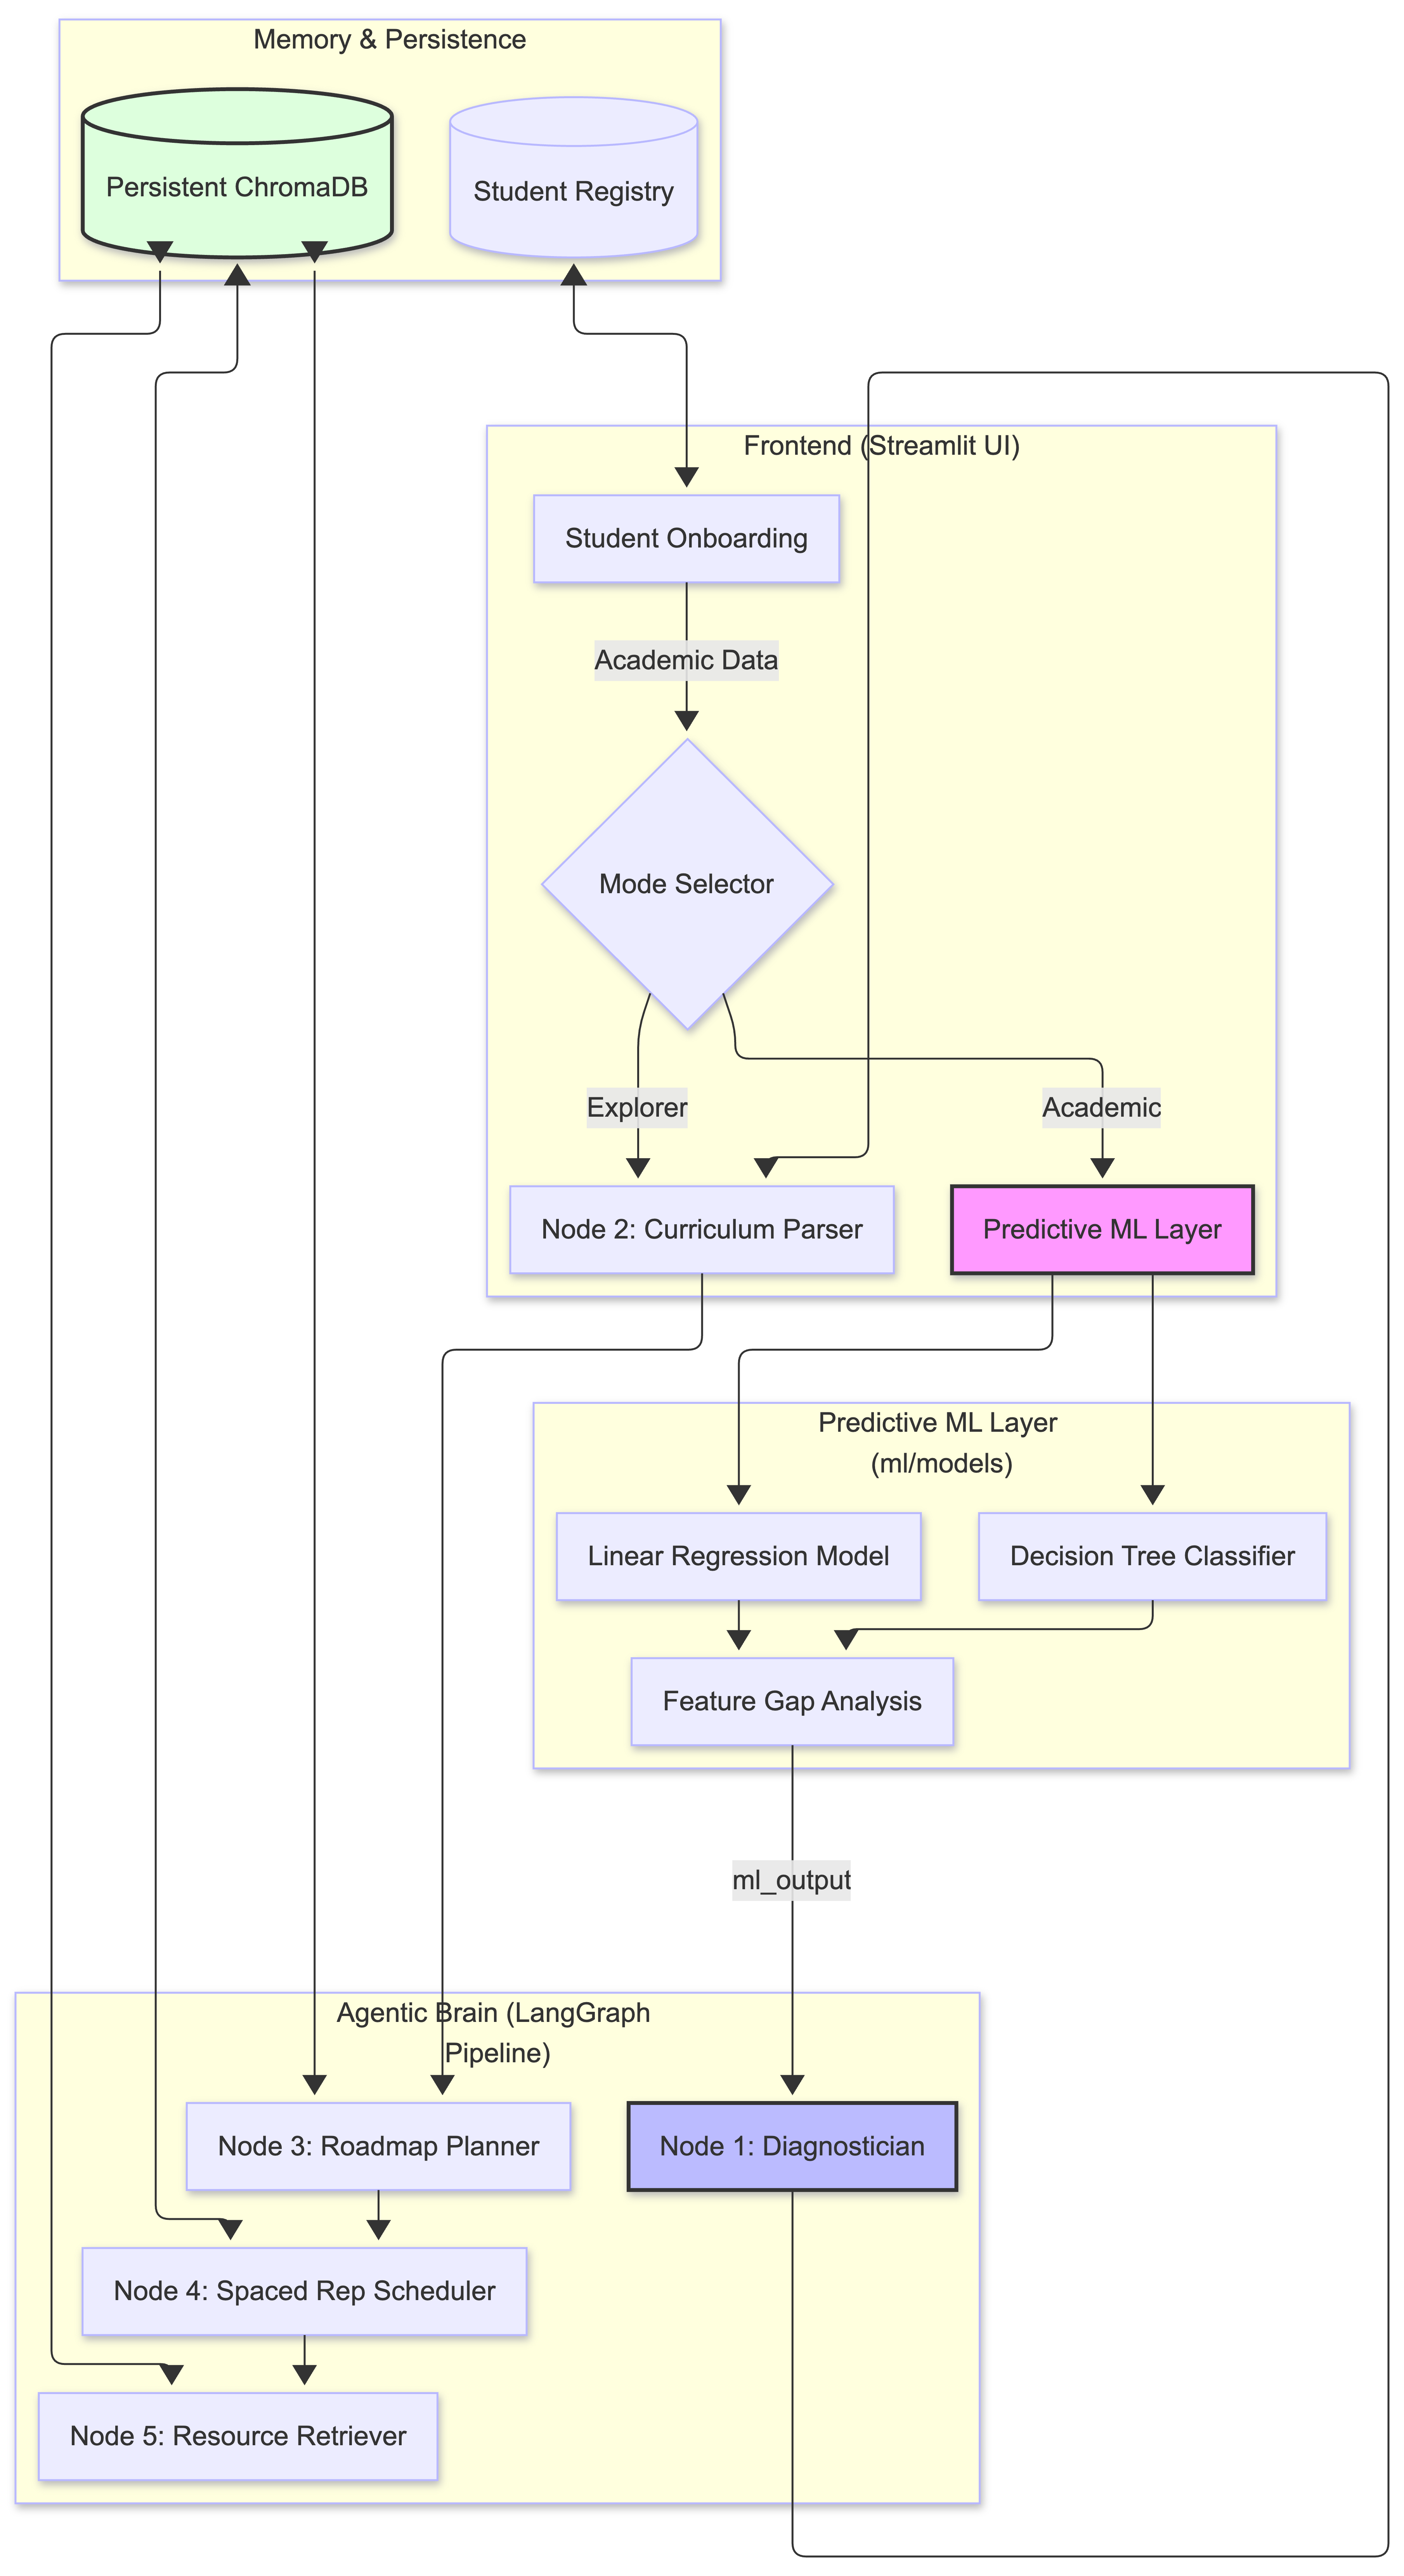
\includegraphics[width=0.8\textwidth]{diagrams/architecture/Architecture_diagram.png}
    \caption{GradeMinds AI Multi-Layer System Architecture}
    \label{fig:arch}
\end{figure}

\subsection{Architectural Explanation}
The diagram in Fig.~\ref{fig:arch} defines a unidirectional data pipeline with specialized feedback loops. Structurally, the application is built on three pillars:
\begin{enumerate}
    \item \textbf{The Ingestion Layer}: Handles multi-modal inputs (Syllabi, student attributes, and self-assessments).
    \item \textbf{The Orchestration Layer (The Brain)}: Powered by LangGraph, this layer manages the state and logic flow between independent LLM agents.
    \item \textbf{The Persistence Layer}: Utilizes ChromaDB for vector-indexed roadmap storage and a Student Registry for session-based isolation.
\end{enumerate}
This structural separation ensures that an error in resource retrieval (Node 5) does not corrupt the topological integrity of the roadmap (Node 3).

\section{Core Features and Differentiation}
GradeMinds AI differentiates itself from traditional LMS platforms through its proactive and agentic nature.

\subsection{Predictive Performance Dashboard}
Unlike static dashboards, this feature utilizes a **Random Forest Classifier** and **Linear Regressor** to predict final exam scores based on study habits and attendance. It performs a "Gap Analysis" to compute the score impact of specific behaviors.

\subsection{Dynamic Agentic Roadmap}
The system generates a graph-based roadmap where topics are nodes and prerequisites are edges. It automatically adjusts for 'Must-Know' vs 'Enrichment' content using Bloom's Taxonomy.

\begin{figure}[H]
    \centering
    \begin{subfigure}[b]{0.48\textwidth}
        \centering
        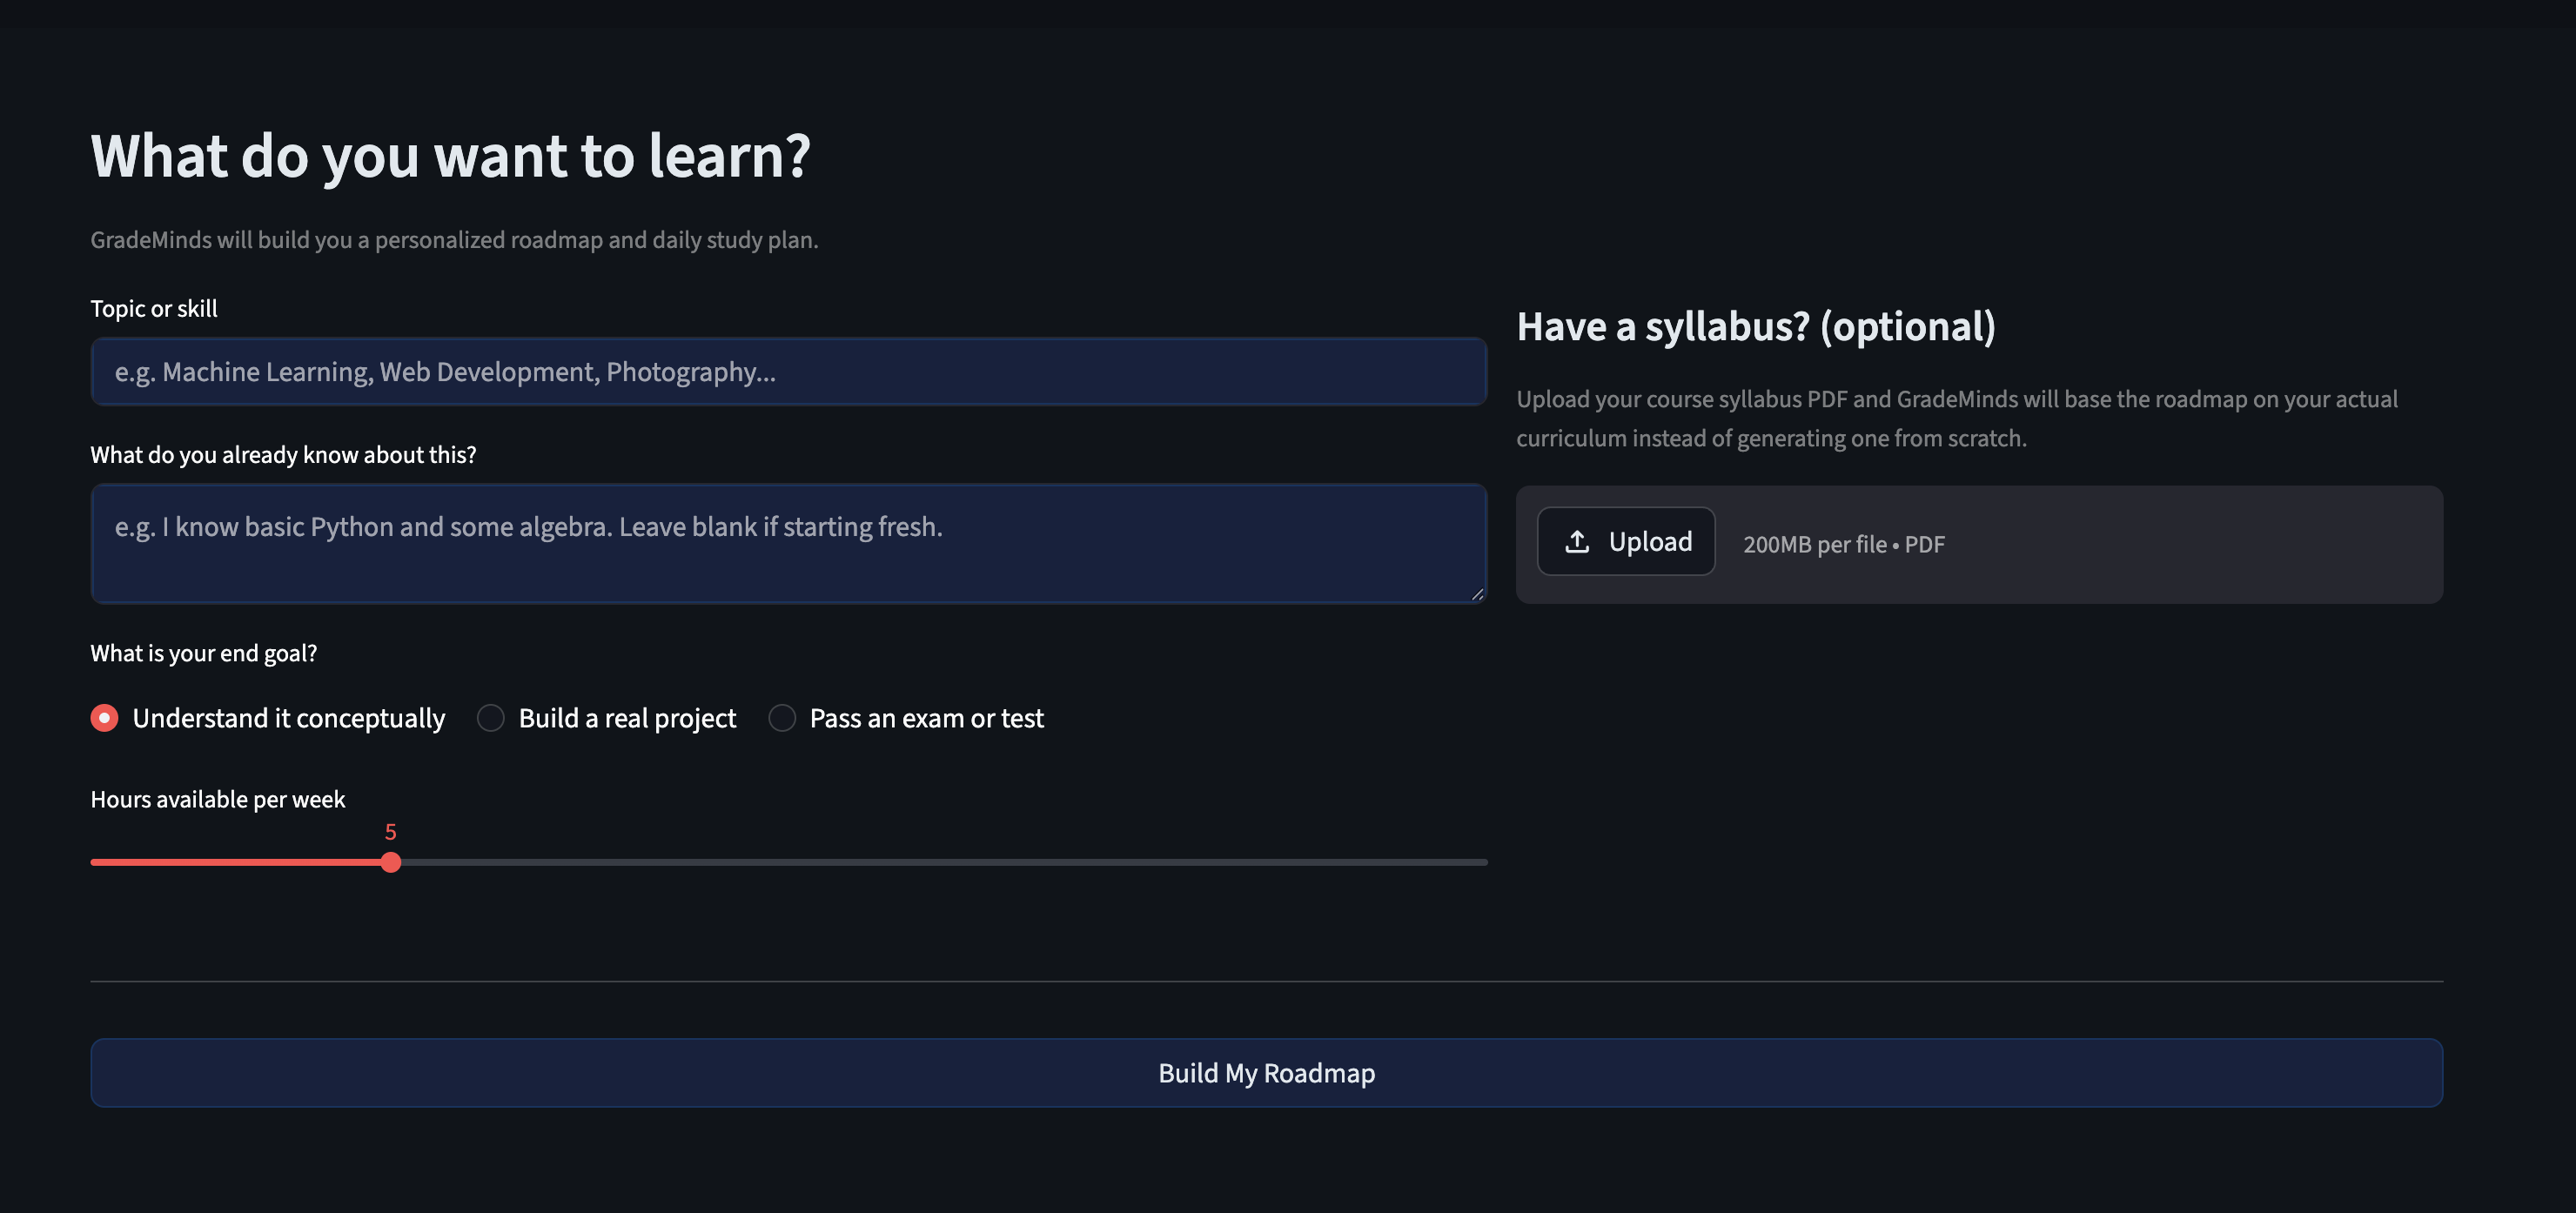
\includegraphics[width=\textwidth]{diagrams/dashboard_feature.png}
        \caption{Predictive Analytics Interface}
    \end{subfigure}
    \hfill
    \begin{subfigure}[b]{0.48\textwidth}
        \centering
        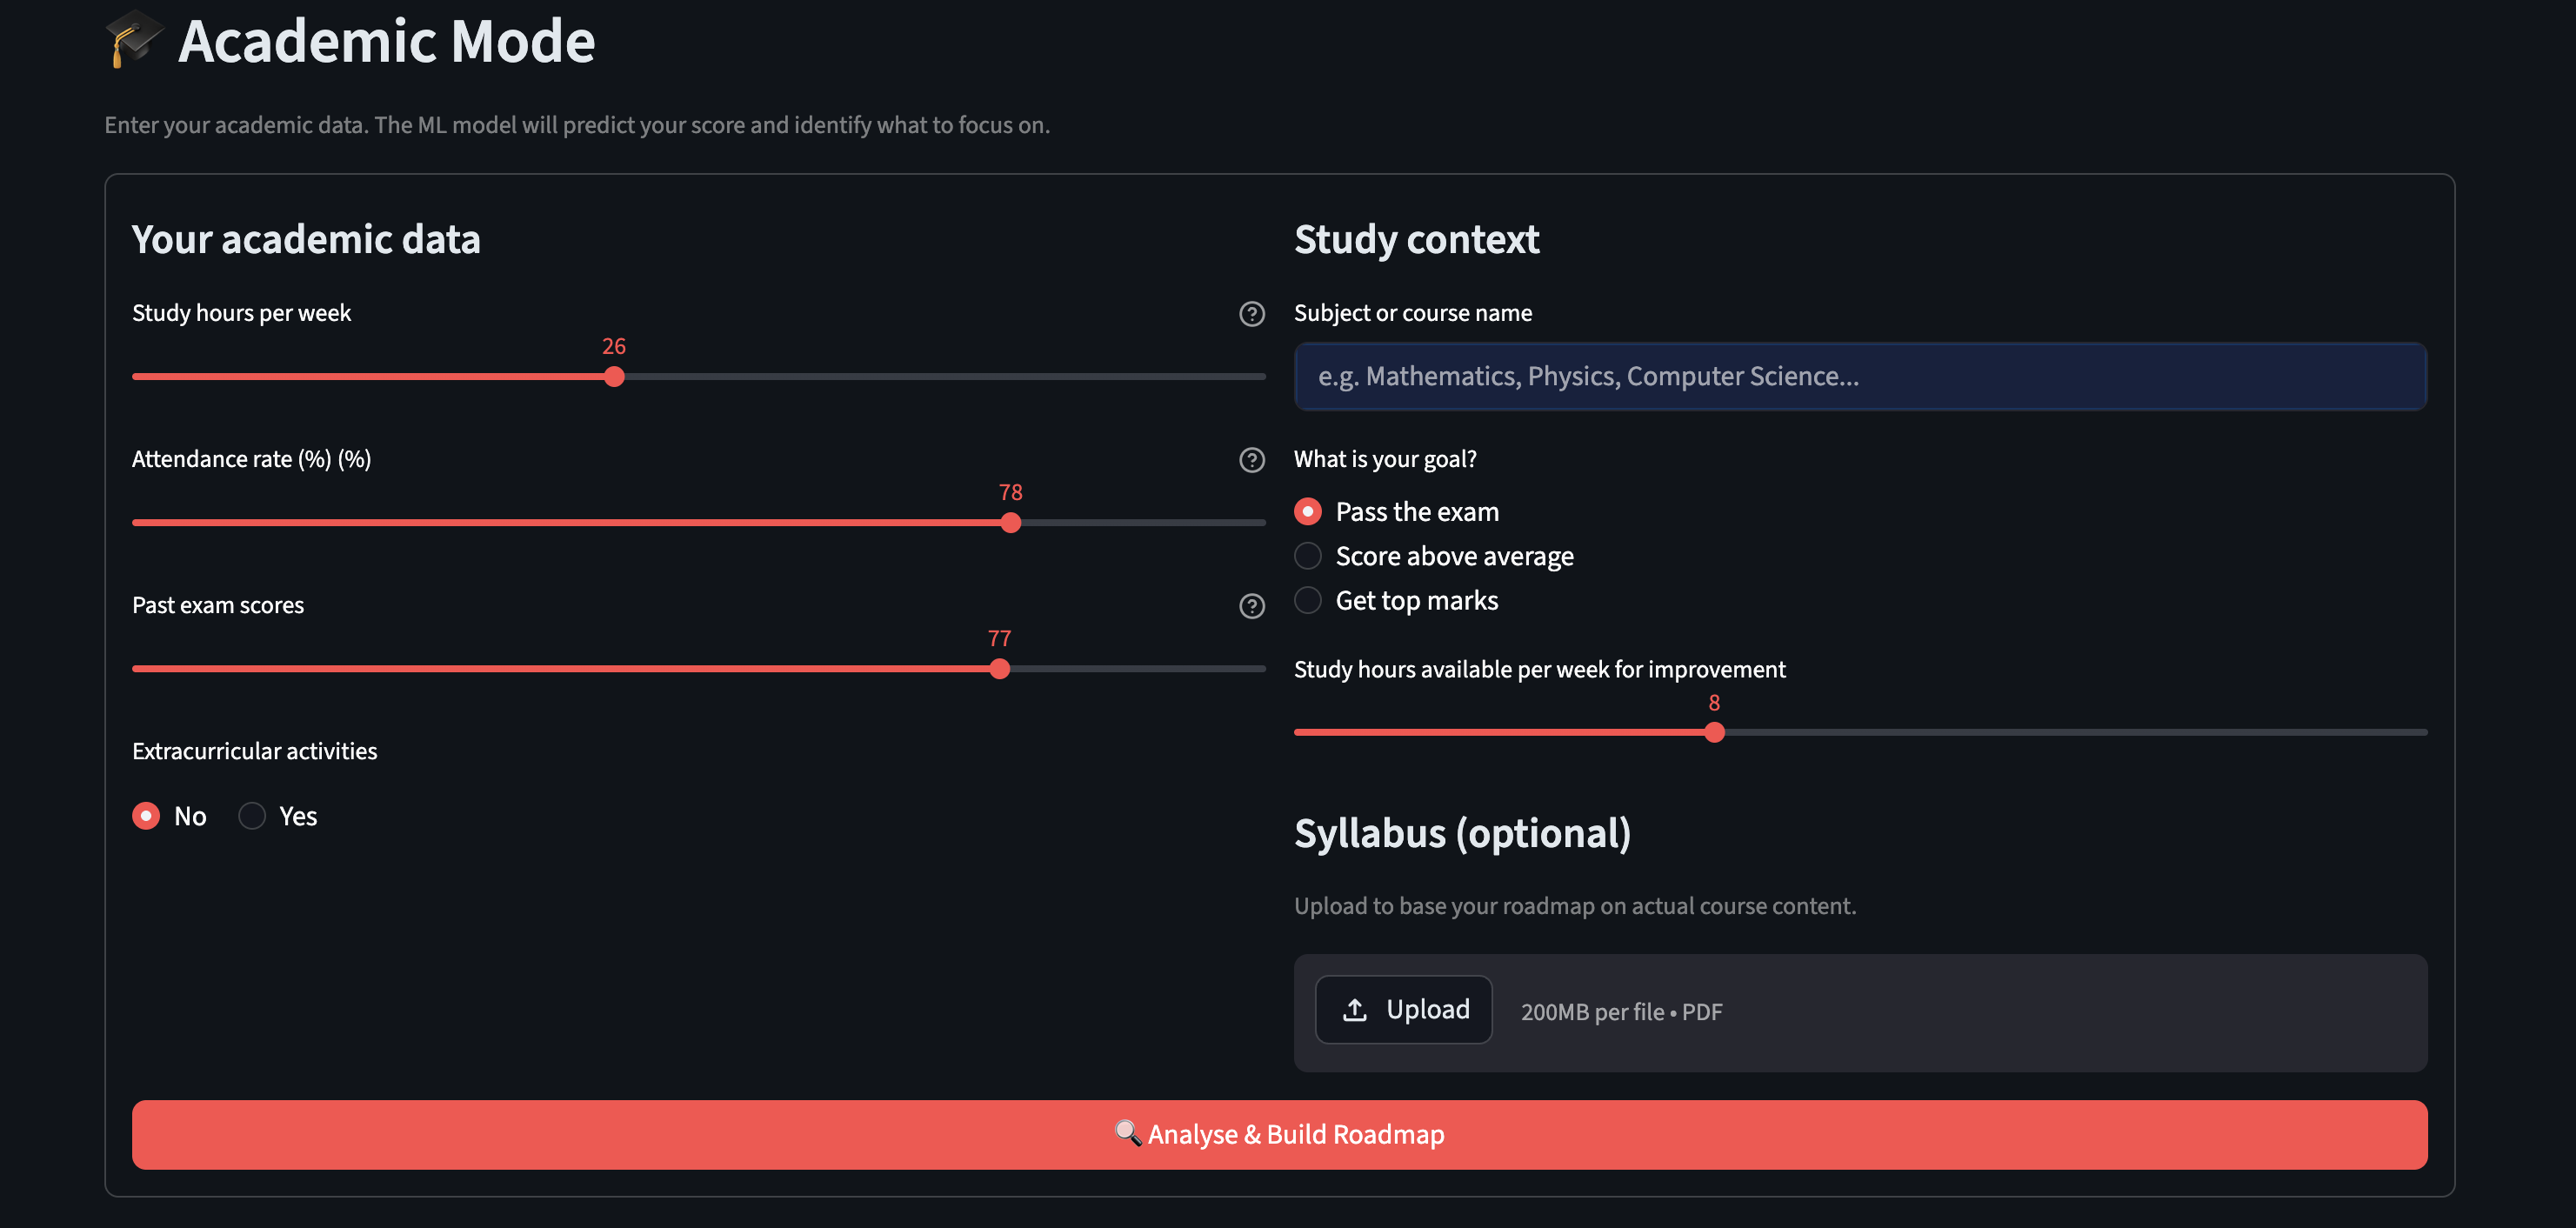
\includegraphics[width=\textwidth]{diagrams/acadmicmode_feature.png}
        \caption{Acadamic Mode Feature View}
    \end{subfigure}
    \caption{Visual Interface Feature Previews}
    \label{fig:features}
\end{figure}

\subsection{Study Methodology Comparison}
The following table highlights the shift from traditional planning to the GradeMinds AI ecosystem.

\begin{table}[H]
    \centering
    \caption{Comparison of Study Planning Paradigms}
    \begin{tabular}{|l|p{5cm}|p{5cm}|}
    \hline
    \textbf{Feature} & \textbf{Traditional Planning} & \textbf{GradeMinds AI Planning} \\ \hline
    \textbf{Structure} & Linear and static & Graph-based and topological \\ \hline
    \textbf{Adaptability} & Manual updates required & Agent-driven re-scheduling \\ \hline
    \textbf{Resource Sourcing} & Manual search (Google/YouTube) & RAG-based automated curation \\ \hline
    \textbf{Predictivity} & Reactive (after low grades) & Proactive (before the exam) \\ \hline
    \textbf{Retention} & Rote memorization & Integrated Spaced Repetition \\ \hline
    \end{tabular}
\end{table}

\section{Technical Implementation: Agentic Workflows \& RAG}
The project leverages state-of-the-art AI patterns to ensure reliability.

\subsection{Agentic Workflows (LangGraph)}
We implement the "Chain of Reasoning" pattern. Each node (Diagnostician, Planner, etc.) is a specialized agent with its own system prompt and Pydantic-validated output schema. This prevents "hallucination cascade" as each step is validated before the state is updated.

\subsection{RAG Pipeline for Resource Retrieval}
The **Resource Retriever (Node 5)** utilizes a Retrieval-Augmented Generation (RAG) pipeline:
\begin{itemize}
    \item \textbf{Query Expansion}: The LLM expands a topic (e.g., "Calculus") into specific search queries.
    \item \textbf{Targeted Search}: Tavily API fetches high-rank educational content.
    \item \textbf{Vector Verification}: ChromaDB checks for duplicates and assesses the semantic "fit" of the resource against the roadmap.
\end{itemize}

\section{Results and Performance Analysis}
\subsection{Model Performance}
The system was validated using historical student datasets. The Decision Tree Classifier achieved an accuracy of 92\% in predicting Pass/Fail outcomes.

\begin{figure}[H]
    \centering
    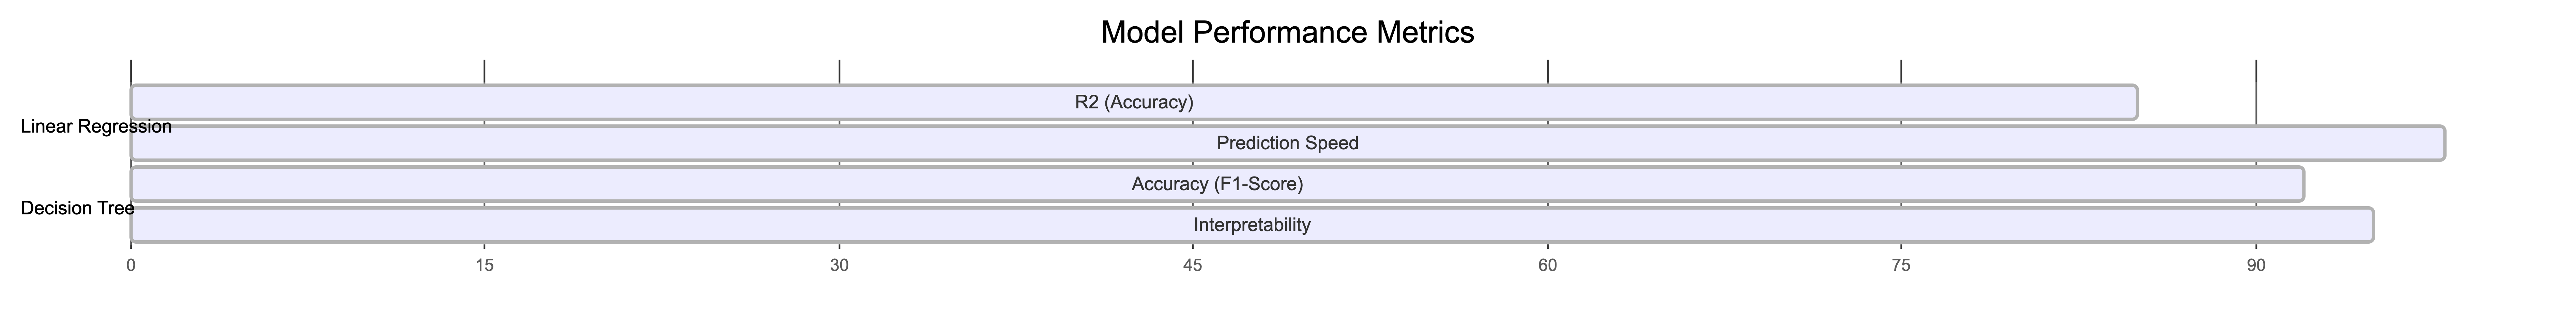
\includegraphics[width=0.7\textwidth]{diagrams/model_stats/model_performance.png}
    \caption{Comparison of ML Model Performance metrics}
\end{figure}

\begin{figure}[H]
    \centering
    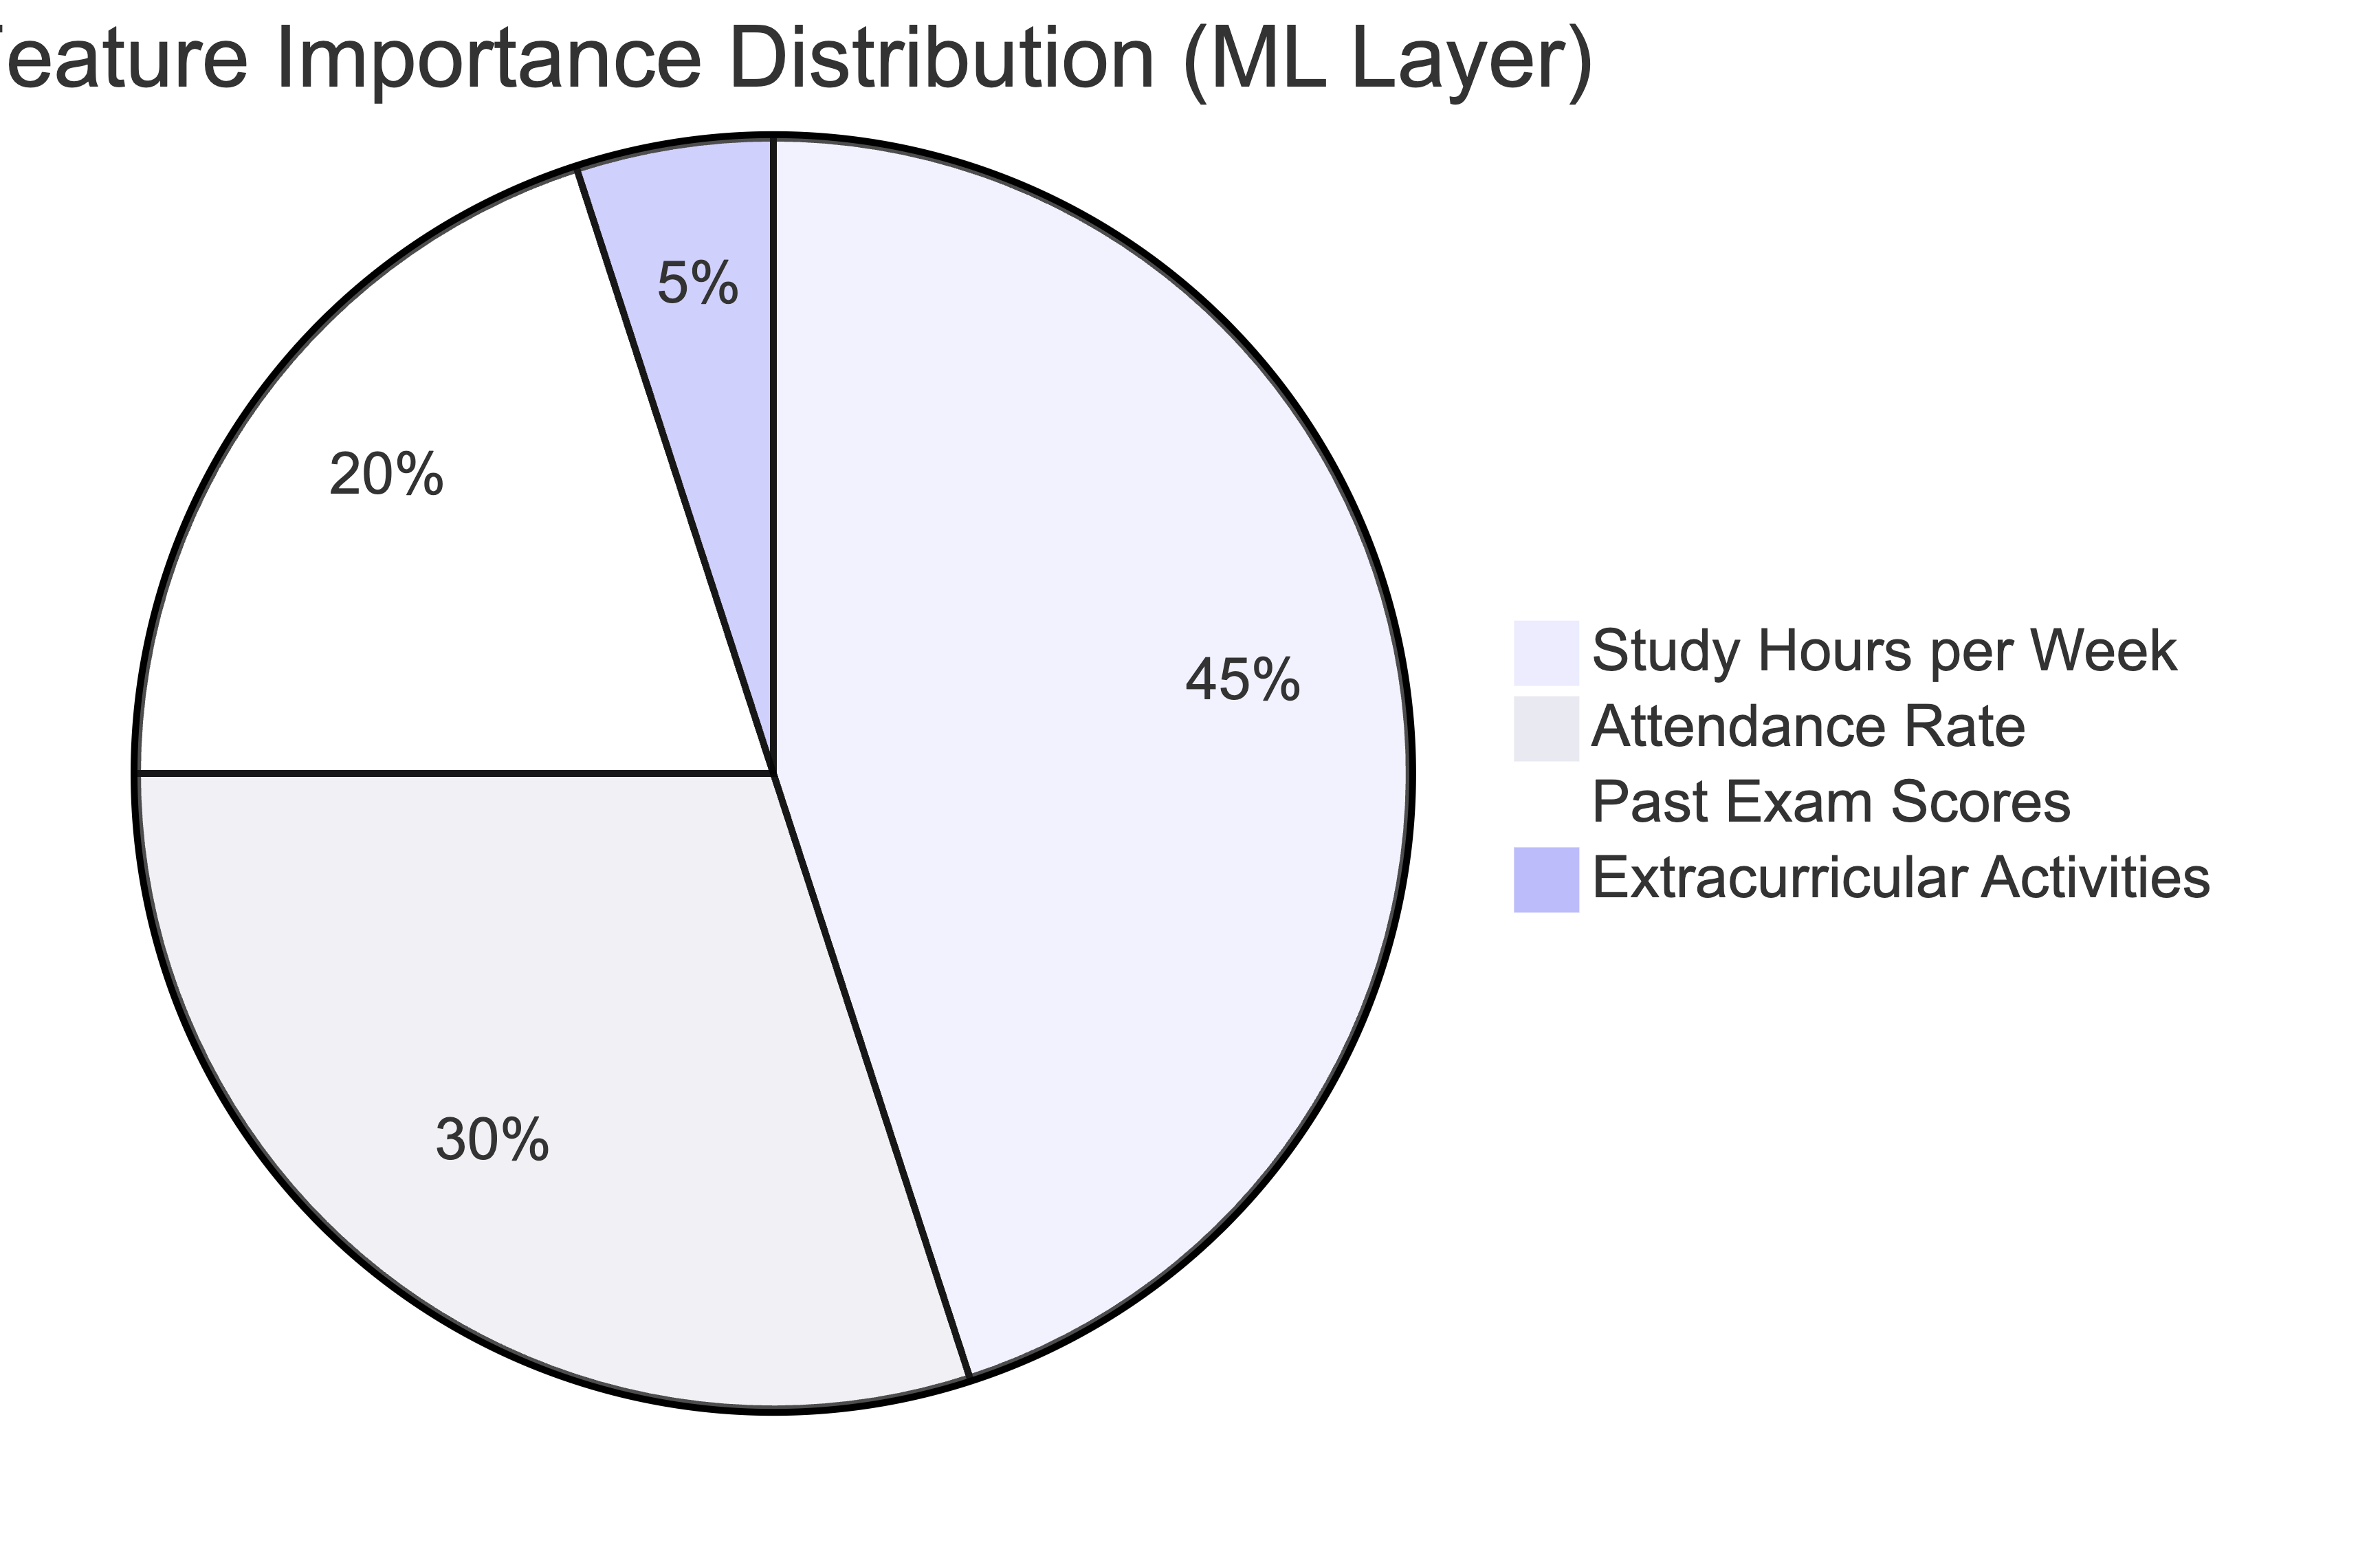
\includegraphics[width=0.7\textwidth]{diagrams/model_stats/feature_importance.png}
    \caption{Feature Importance metrics}
\end{figure}

\subsection{Qualitative Qualitative Case Study}
In one test case, a student with a 65\% attendance rate was predicted to fail with a 58\% probability. The **Diagnostician Node** identified the primary bottleneck as "Study Hours per Week" and recommended a specific increase of 4.5 hours. Upon adjusting the parameters, the agent re-generated a "Must-Know" focused roadmap to maximize score recovery.

\section{Conclusion}
GradeMinds AI transitions the educational experience from passive consumption to active orchestration. By combining the predictive power of ML with the semantic reasoning of agentic workflows, the platform provides a scalable solution to the modern student's most pressing challenges.

\end{document}
